% !TEX encoding = UTF-8 Unicode
%!TEX TS-program = xelatex

\documentclass[12pt]{extarticle}
% extarticle is like article but can handle 8pt, 9pt, 10pt, 11pt, 12pt, 14pt, 17pt, and 20pt text

\def \ititle {Origins of Mind}
 
\def \isubtitle {Lecture 08}
 
\def \iauthor {Stephen A. Butterfill}
\def \iemail{s.butterfill@warwick.ac.uk}
\date{}

%for strikethrough
\usepackage[normalem]{ulem}

\usepackage{pdfpages}


\input{$HOME/Documents/submissions/preamble_steve_handout}

%logic symbol \leftmodels
\usepackage{MnSymbol}

%\bibpunct{}{}{,}{s}{}{,}  %use superscript TICS style bib
%remove hanging indent for TICS style bib
%TODO doesnt work
\setlength{\bibhang}{0em}
%\setlength{\bibsep}{0.5em}


%itemize bullet should be dash
\renewcommand{\labelitemi}{$-$}

\begin{document}

%\raggedcolumns

\begin{multicols*}{3}

\setlength\footnotesep{1em}


\bibliographystyle{newapa} %apalike

%\maketitle
%\tableofcontents




%--------------- 
%--- start paste
\def \ititle {Logic I}
 
\def \isubtitle {Lecture 1}
 
\begin{center}
 
{\Large
 
\textbf{\ititle}: \isubtitle
 
}
 
 
 
\iemail %
 
\end{center}
 
Readings refer to sections of the course textbook, \emph{Language, Proof and Logic}.
 
 
 
\section{Quick Intro to FOL}
 
\emph{Reading:} §1.1, §1.2, §1.3
 
\begin{center}
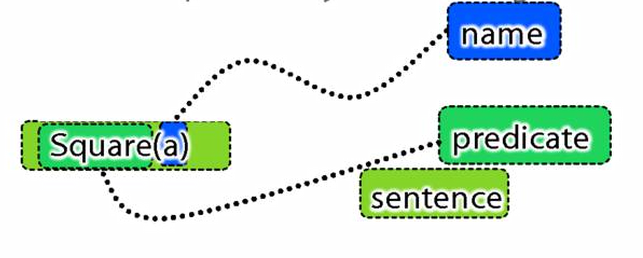
\includegraphics[scale=0.3]{img/name_predicate_sentence.png}
\end{center}
A formal langauge enables us to avoid ambiguity, e.g.:
 
\begin{quote}
 
This is a hospital where doctors are trained.
 
\end{quote}
 
A formal langauge also enables us to some avoid appearance--reality problems:
 
\begin{quote}
 
Many more people have been to Paris than I have.
 
\end{quote}
 
 
 
\section{Logically Valid Arguments}
 
\emph{Reading:} §2.1
 
An argument is \emph{logically valid} just if there’s no possible situation in which the premises are true and the conclusion false
 
A \emph{connective} joins one or more sentences to make a new sentence. E.g. ‘because’, ‘¬’. The sentences joined by a connective are called \emph{constituent sentences}.
 
E.g. in ‘P $\lor{}$ Q’,
 
\begin{quote}
 
$\lor{}$ is the connective
 
P, Q are the constituent sentences
 
\end{quote}
 
\begin{center}
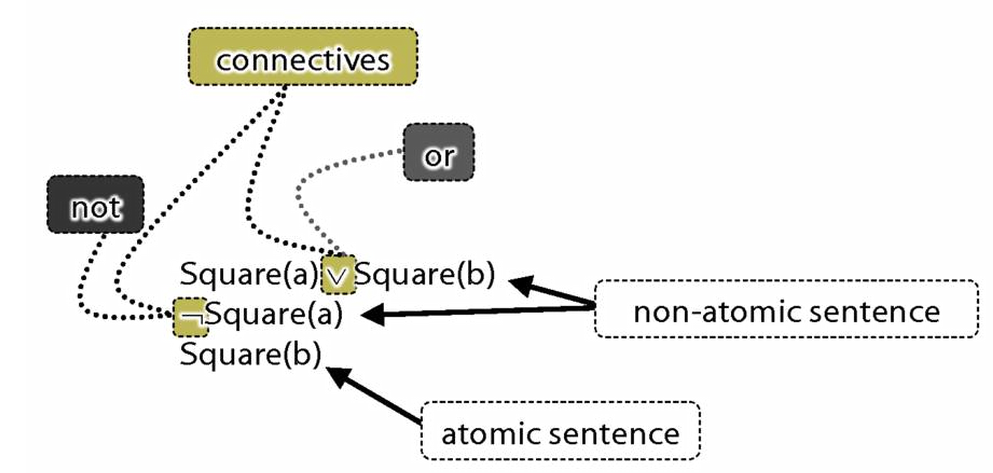
\includegraphics[scale=0.3]{img/terminology_more.png}
\end{center}
 
 
\section{Counterexamples}
 
\emph{Reading:} §2.5
 
A \emph{counterexample} to an argument is a possible situation in which its premises are T and its conclusion F.
 
There are no counterexamples to a logically valid argument.
 
If an argument is not valid, then there is a counterexample to it.
 
To show that an argument is not logically valid, we specify a counterexample to it.
 
 
 
\section{Identity}
 
\emph{Reading:} §2.2
 
Principle: If b=c then whatever is true of b is also true of c.
 
Principle: a=a is never false
 
\begin{center}
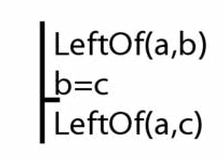
\includegraphics[scale=0.3]{img/arg_identity.png}
\end{center}
 
 
\section{Sentence Letters}
 
\begin{center}
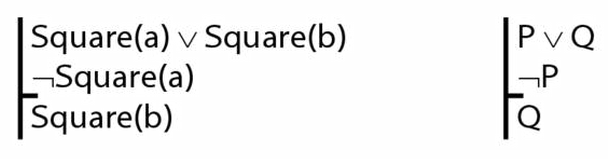
\includegraphics[scale=0.3]{img/sentence_letters.png}
\end{center}
 
 
\section{Truth Tables}
 
\emph{Reading:} §3.1, §3.2, §3.3
 
Rough guide:
 
`$\land{}$' means and
 
`$\lor{}$' means or
 
`$\lnot{}$' means not
 
\begin{center}
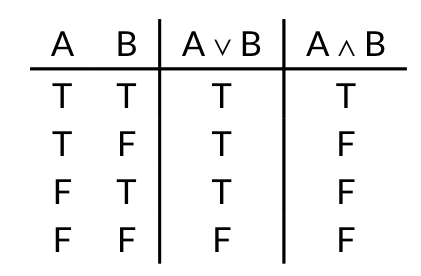
\includegraphics[scale=0.3]{img/truth_table_or_and.png}
\end{center}
\begin{center}
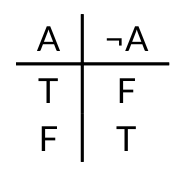
\includegraphics[scale=0.3]{img/truth_table_not.png}
\end{center}
 
 
\section{Complex Truth Tables}
 
\begin{center}
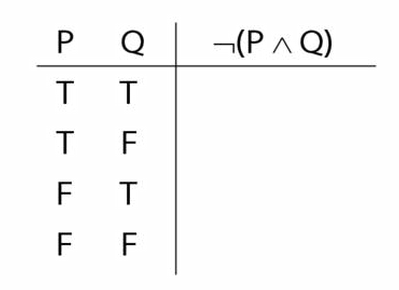
\includegraphics[scale=0.3]{img/unit_60_tt.png}
\end{center}
\vfill
%\begin{minipage}{\columnwidth}
%\section{Exercises}
%These exercises will be discussed in seminars the week after this lecture.
%The numbers below refer to the numbered exercises in the course textbook, e.g.\ `1.1' refers to exercise 1.1. on page 39 of the second edition of \emph{Language, Proof and Logic}. Exercises marked `*' are optional.
% 
%\begin{quote}
%1.1--1.5
% 
%*1.6
% 
%1.8--1.10
% 
%2.3, 2.4
% 
%2.8, 2.10, 2.12, 2.21
% 
%2.5, 2.6
% 
%3.1, 3.2
% 
%3.5, 3.7
% 
%\end{quote}
%\end{minipage}
%--- end paste
%--------------- 
 


\end{multicols*}

\end{document}